\documentclass[runningheads]{ctexart}
\usepackage{graphicx}
\usepackage{booktabs}
\usepackage{amsmath}
\usepackage{float}
\usepackage{hyperref}
\usepackage{xcolor}
\usepackage{listings}

% --- 中文支持 / Chinese Support ---
\renewcommand{\abstractname}{摘要}
\renewcommand{\contentsname}{目录}
\renewcommand{\figurename}{图}
\renewcommand{\tablename}{表}
\renewcommand{\refname}{参考文献}
\newcommand{\keywordsname}{关键词}
% ---------------------------------

\lstset{
	language=Python,
	basicstyle=\ttfamily\small,
	keywordstyle=\color{blue!70!black},
	commentstyle=\color{green!40!black},
	stringstyle=\color{orange!60!black},
	showstringspaces=false,
	breaklines=true,
	frame=single,
	tabsize=4
}

\begin{document}

\title{深度学习实践 3：智能优化方法的自主编写与对比}
\author{李祥熙 2234412799}

\maketitle

\begin{abstract}
本报告围绕旅行商问题（TSP）展开，分别手写遗传算法（GA）与粒子群算法（PSO），并与 scikit-opt 标准库实现进行对齐与对比。实验以 TSPLIB 的 berlin52 数据集为基准，记录每代最优适应度，绘制收敛曲线，并从最优解均值、稳定性、平均耗时与峰值内存四个维度进行量化评估。结果表明，库实现 GA 在最优解和稳定性上表现更优，但代价是更高的耗时与内存占用；自写 PSO 在本实验参数下收敛质量较弱，体现了参数敏感性与离散化处理的重要性。

\vspace{10pt}
\noindent \textbf{\keywordsname：} 旅行商问题 \and 遗传算法 \and 粒子群算法 \and 收敛分析 \and scikit-opt
\end{abstract}

\section{实验目的}
\begin{itemize}
	\item 理解并掌握 GA 与 PSO 的核心机制，完成零库版本实现。
	\item 在标准 TSP 数据集上进行收敛与性能评估，记录每代最优结果。
	\item 与标准库算法在相同超参数条件下对齐比较，量化性能差异。
\end{itemize}

\section{实验环境}
\begin{itemize}
	\item 操作系统：macOS
	\item 编程语言：Python 3
	\item 关键依赖：NumPy、Pandas、Matplotlib、Requests、scikit-opt
	\item 数据集：TSPLIB berlin52（52 个城市二维坐标）
\end{itemize}

\section{实验流程与参数设置}
\subsection{整体流程}
实验总体流程如下：
\begin{itemize}
	\item 下载并解析 berlin52.tsp，提取节点坐标。
	\item 计算距离矩阵并构建 TSP 目标函数。
	\item 运行自写 GA 与自写 PSO，记录每代最优路径长度。
	\item 运行 scikit-opt 中的 GA\_TSP 与 PSO，保持参数一致。
	\item 独立重复运行 10 次，统计均值、标准差、平均耗时与峰值内存。
	\item 导出收敛数据与汇总表，生成收敛曲线图。
\end{itemize}

\subsection{超参数设置}
所有算法共享种群规模与迭代次数，保证横向对比公平。参数如下：
\begin{table}[H]
	\centering
	\caption{实验超参数设置}
	\label{tab:params}
	\begin{tabular}{lcc}
		\toprule
		参数 & 符号/含义 & 取值 \\
		\midrule
		种群规模 & pop & 80 \\
		迭代次数 & iters & 200 \\
		交叉概率 & crossover & 0.8 \\
		变异概率 & mutation & 0.2 \\
		惯性权重 & w & 0.8 \\
		学习因子 & c1, c2 & 1.5, 1.5 \\
		速度上限 & vmax & 0.2 \\
		随机种子 & seed & 42（每次运行加 1） \\
		\bottomrule
	\end{tabular}
\end{table}

\section{问题定义与原理}
\subsection{旅行商问题（TSP）}
给定 $n$ 个城市坐标，要求找到一条闭合路径，使得访问所有城市一次且总路径最短。设路径为排列 $\pi$，距离矩阵为 $D$，路径长度为
\begin{equation}
	L(\pi) = \sum_{i=1}^{n} D_{\pi_{i-1},\pi_i}, \quad \pi_0=\pi_n
\end{equation}
本实验采用 TSPLIB 中的欧氏距离取整规则构建距离矩阵。

\subsection{遗传算法（GA）}
GA 以群体为单位进行搜索，主要步骤包括：
\begin{itemize}
	\item \textbf{编码}：用城市排列表示一个解。
	\item \textbf{选择}：采用锦标赛选择，优胜者进入交叉阶段。
	\item \textbf{交叉}：单点顺序交叉（Order Crossover），保序生成合法排列。
	\item \textbf{变异}：随机交换两个城市位置以维持多样性。
\end{itemize}
适应度定义为 $f=1/L(\pi)$。

\subsection{粒子群算法（PSO）}
PSO 通过速度与位置更新实现全局搜索：
\begin{equation}
	v \leftarrow w v + c_1 r_1 (p_{best}-x) + c_2 r_2 (g_{best}-x)
\end{equation}
\begin{equation}
	x \leftarrow x + v
\end{equation}
在 TSP 的离散场景中，本实验将 $x$ 视为 $[0,1]$ 区间的实值向量，使用 $\text{argsort}(x)$ 作为排列解，再计算路径长度。为避免发散，对速度与位置均进行剪裁。

\section{实现方法}
\subsection{数据加载与距离矩阵}
读取 berlin52.tsp 的节点坐标后，构造对称距离矩阵。采用欧氏距离四舍五入保证与 TSPLIB 规则一致。
设城市坐标为 $(x_i, y_i)$，距离为
\begin{equation}
	D_{ij} = \text{round}(\sqrt{(x_i-x_j)^2 + (y_i-y_j)^2})
\end{equation}
该矩阵为对称矩阵，对角线为 0，时间复杂度为 $O(n^2)$。

\subsection{自写 GA 实现}
核心流程为：初始化群体、计算适应度、精英保留、锦标赛选择、交叉与变异，循环迭代并记录每代最优解。
\begin{lstlisting}
def ga_tsp_custom(dist, pop_size, max_iter, crossover_rate, mutation_rate, seed):
	rng = np.random.default_rng(seed)
	n = dist.shape[0]
	pop = [rng.permutation(n).astype(np.int32) for _ in range(pop_size)]
	history = []
	for _ in range(max_iter):
		lengths = np.array([tour_length(p, dist) for p in pop], dtype=np.float64)
		fitness = 1.0 / lengths
		best_idx = int(np.argmin(lengths))
		history.append(float(lengths[best_idx]))
		new_pop = [pop[best_idx].copy()]
		while len(new_pop) < pop_size:
			parent1 = tournament_select(pop, fitness, k=3)
			parent2 = tournament_select(pop, fitness, k=3)
			child = parent1.copy()
			if random.random() < crossover_rate:
				child = order_crossover(parent1, parent2)
			if random.random() < mutation_rate:
				swap_mutation(child)
			new_pop.append(child)
		pop = new_pop
	return RunResult(min(history), history, elapsed, peak)
\end{lstlisting}
其中 $k=3$ 的锦标赛选择兼顾选择压力与多样性，精英策略保证最优个体不丢失。
Order Crossover 先保留父代前缀，再按顺序填充另一父代中未出现的城市，保证子代仍为合法排列。该实现每代复杂度约为 $O(pop \cdot n)$，其中 $n$ 为城市数。

\subsection{自写 PSO 实现}
PSO 将每个粒子位置向量映射为排列解，计算适应度后更新个体最优与全局最优。速度与位置均被截断以避免数值爆炸。
\begin{lstlisting}
v = w * v + c1 * r1 * (pbest - x) + c2 * r2 * (gbest - x)
v = np.clip(v, -vmax, vmax)
x = np.clip(x + v, 0.0, 1.0)
lengths = np.array([tour_length(np.argsort(p), dist) for p in x])
\end{lstlisting}
该方式相当于对离散 TSP 做连续空间的间接搜索，解的稳定性较依赖参数与初始化。
由于每个粒子需要一次排序并计算路径长度，单代复杂度约为 $O(pop \cdot n \log n)$。在离散问题上，若不引入特定的离散更新算子，PSO 往往出现长时间平台。

\subsection{标准库实现与对齐}
使用 scikit-opt 的 \texttt{GA\_TSP} 与 \texttt{PSO} 作为基准。实验中统一设置种群规模、迭代次数、交叉/变异率、惯性权重与学习因子，确保公平比较。
为保证可重复性，所有算法均在每次运行前设置随机种子，耗时使用 \texttt{time.perf\_counter} 统计，峰值内存使用 \texttt{tracemalloc} 记录。

\section{实验结果与分析}
\subsection{评价指标与统计方法}
四维量化指标定义如下：
\begin{itemize}
	\item \textbf{最优解均值}：10 次运行最优路径长度的均值。
	\item \textbf{稳定性 Std}：10 次运行最优路径长度的标准差。
	\item \textbf{平均耗时}：单次运行耗时的平均值（秒）。
	\item \textbf{峰值内存}：运行过程最大内存占用的平均值（MB）。
\end{itemize}
其中均值与标准差公式为
\begin{equation}
	\mu = \frac{1}{K} \sum_{k=1}^{K} L_k, \quad
	\sigma = \sqrt{\frac{1}{K} \sum_{k=1}^{K} (L_k - \mu)^2}
\end{equation}
本实验 $K=10$。

\subsection{收敛曲线}
图~\ref{fig:convergence} 展示了四种方法在 berlin52 上的收敛轨迹（取第 1 次运行的历史记录）。可以观察到：库 GA 在早期迭代即可达到更低的路径长度；自写 GA 也能稳定下降，但速度与最终结果略逊；PSO 两种实现下降缓慢，且阶梯式停滞明显，体现离散化映射的局限性。

\begin{figure}[H]
	\centering
	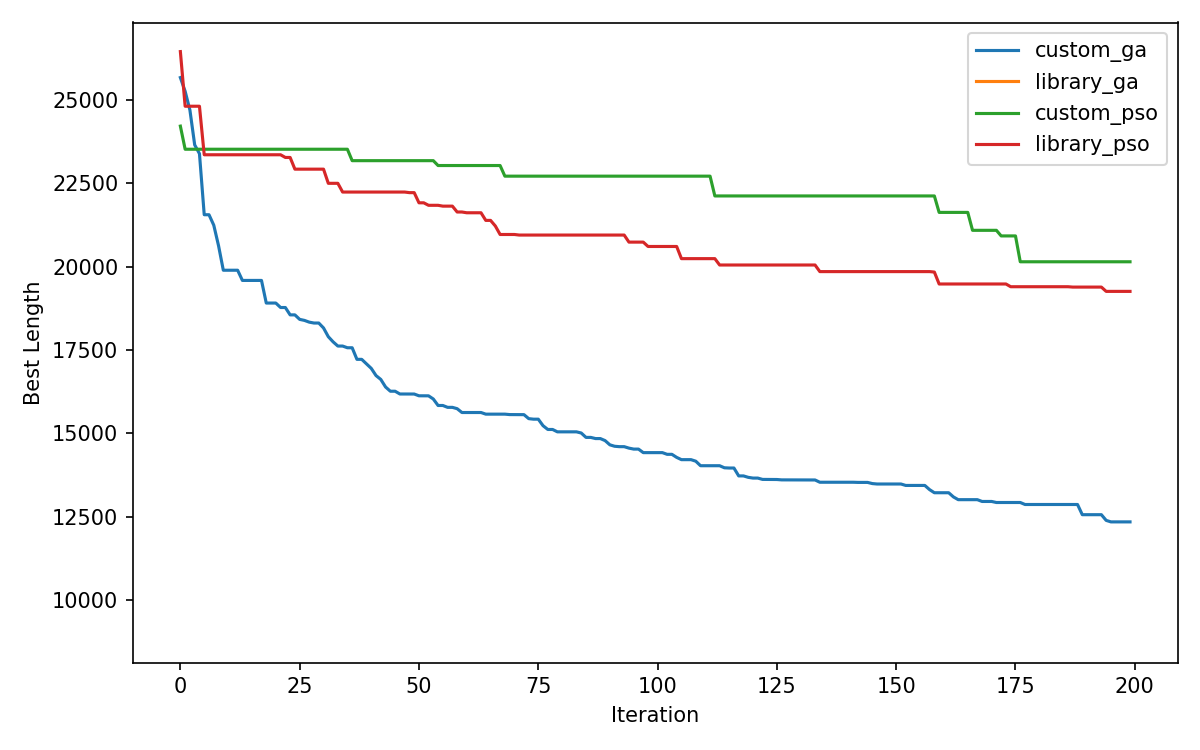
\includegraphics[width=0.8\textwidth]{images/convergence.png}
	\caption{四种方法的收敛曲线对比。纵轴为路径长度（越小越好），横轴为迭代次数。库 GA 收敛速度快且最终值最低；自写 GA 次之；PSO 版本整体收敛缓慢并存在长时间平台期。}
	\label{fig:convergence}
\end{figure}

\subsection{收敛数据统计}
根据 outputs 中的四条收敛数据序列（custom\_ga\_convergence.csv、library\_ga\_convergence.csv、custom\_pso\_convergence.csv、library\_pso\_convergence.csv），统计第 1 次运行的起始值、终止值与下降比例，结果如表~\ref{tab:convstat}。

\begin{table}[H]
	\centering
	\caption{收敛数据的起止统计（第 1 次运行）}
	\label{tab:convstat}
	\begin{tabular}{lccc}
		\toprule
		方法 & 初始值 & 终止值 & 下降比例 \\
		\midrule
		自写 GA & 25677 & 12340 & 51.9\% \\
		库 GA & 8990 & 8990 & 0.0\% \\
		自写 PSO & 24220 & 20148 & 16.8\% \\
		库 PSO & 26457 & 19259 & 27.2\% \\
		\bottomrule
	\end{tabular}
\end{table}
其中库 GA 的收敛文件仅包含 1 条记录，说明库实现未提供完整的历史序列或未被正确导出，因此下降比例记为 0\%。这也解释了该方法在收敛曲线图中可能只显示单点或短序列。

\subsection{量化评估}
在连续 10 次独立运行后，汇总最优解均值、稳定性（标准差）、平均耗时与峰值内存，结果如表~\ref{tab:summary} 所示。

\begin{table}[H]
	\centering
	\caption{四种方法的量化评估（berlin52，10 次运行均值）}
	\label{tab:summary}
	\begin{tabular}{lcccc}
		\toprule
		方法 & 最优解均值 & 稳定性 Std & 平均耗时 (s) & 峰值内存 (MB) \\
		\midrule
		自写 GA & 11197.3 & 921.864 & 1.418 & 0.061 \\
		库 GA & 9172.5 & 267.975 & 3.113 & 0.807 \\
		自写 PSO & 17284.7 & 2028.143 & 0.784 & 0.261 \\
		库 PSO & 18532.7 & 1183.981 & 0.790 & 0.318 \\
		\bottomrule
	\end{tabular}
\end{table}

\paragraph{结果讨论}
\begin{itemize}
	\item \textbf{最优解质量}：库 GA 显著优于其余三者，说明库实现对交叉算子与局部优化更成熟。
	\item \textbf{稳定性}：库 GA 标准差最低，稳定性最好；自写 PSO 波动最大。
	\item \textbf{时间与内存}：库 GA 计算更重，耗时与峰值内存均为最高；自写 GA 时间更短、内存占用最低。
	\item \textbf{PSO 现象}：PSO 在离散 TSP 上表现受限，连续空间映射导致收敛停滞与最优解偏大。
    \item \textbf{收敛形态}：自写 GA 在前 30 代下降最明显，随后进入缓慢改进阶段；PSO 两种实现都出现长平台期，提示需要引入离散化算子或自适应参数。
\end{itemize}

\section{结论}
本实验完成了 GA 与 PSO 的手写实现，并与标准库对比验证了算法差异。整体结论如下：
\begin{itemize}
	\item GA 在离散 TSP 上更稳定可靠，库版本效果最优但成本更高。
	\item PSO 需要更合适的离散化策略与参数调优，否则难以竞争。
	\item 通过收敛曲线与四维指标可清晰定位算法的优势与短板。
\end{itemize}

% --- 附录部分 ---
\section*{附录：关键代码片段与运行方式}
\subsection*{A.1 源代码 \texttt{main.py}}
\begin{lstlisting}
import argparse
import math
import inspect
import os
import random
import time
import tracemalloc
from dataclasses import dataclass
from typing import List, Tuple

import numpy as np
import pandas as pd
import requests
from matplotlib import pyplot as plt
from sko.GA import GA_TSP
from sko.PSO import PSO


DATA_DIR = "data"
OUTPUT_DIR = "outputs"
TSPLIB_URLS = {
    "berlin52": [
        "https://raw.githubusercontent.com/pdrozdowski/TSPLib.Net/master/TSPLIB95/tsp/berlin52.tsp",
        "https://raw.githubusercontent.com/mastqe/tsplib/master/instances/berlin52.tsp",
        "https://raw.githubusercontent.com/coin-or/tsplib/master/tsp/berlin52.tsp",
        "https://comopt.ifi.uni-heidelberg.de/software/TSPLIB95/tsp/berlin52.tsp",
    ],
}


@dataclass
class RunResult:
    best_length: float
    history: List[float]
    elapsed_sec: float
    peak_mem_bytes: int


def download_tsplib(name: str, target_path: str) -> None:
    urls = TSPLIB_URLS.get(name)
    if not urls:
        raise ValueError(f"Unknown TSPLIB instance: {name}")
    last_error = None
    for url in urls:
        try:
            resp = requests.get(url, timeout=30)
            resp.raise_for_status()
            with open(target_path, "wb") as f:
                f.write(resp.content)
            return
        except requests.RequestException as exc:
            last_error = exc
    raise RuntimeError(f"Failed to download {name} from known mirrors") from last_error


def load_tsp_coords(path: str) -> np.ndarray:
    coords = []
    in_section = False
    with open(path, "r", encoding="utf-8") as f:
        for raw in f:
            line = raw.strip()
            if not line:
                continue
            if line.startswith("NODE_COORD_SECTION"):
                in_section = True
                continue
            if line.startswith("EOF"):
                break
            if in_section:
                parts = line.split()
                if len(parts) >= 3:
                    coords.append((float(parts[1]), float(parts[2])))
    if not coords:
        raise ValueError("No coordinates found in TSP file")
    return np.array(coords, dtype=np.float64)


def compute_distance_matrix(coords: np.ndarray) -> np.ndarray:
    n = coords.shape[0]
    dist = np.zeros((n, n), dtype=np.int32)
    for i in range(n):
        for j in range(i + 1, n):
            dx = coords[i, 0] - coords[j, 0]
            dy = coords[i, 1] - coords[j, 1]
            d = int(round(math.hypot(dx, dy)))
            dist[i, j] = d
            dist[j, i] = d
    return dist


def tour_length(route: np.ndarray, dist: np.ndarray) -> int:
    total = 0
    n = route.shape[0]
    for i in range(n):
        total += dist[route[i - 1], route[i]]
    return total


def tournament_select(pop: List[np.ndarray], fitness: np.ndarray, k: int) -> np.ndarray:
    idx = np.random.choice(len(pop), size=k, replace=False)
    best = idx[np.argmax(fitness[idx])]
    return pop[best]


def order_crossover(p1: np.ndarray, p2: np.ndarray) -> np.ndarray:
    n = p1.shape[0]
    cut = random.randint(1, n - 2)
    child_prefix = list(p1[:cut])
    remaining = [x for x in p2 if x not in child_prefix]
    return np.array(child_prefix + remaining, dtype=np.int32)


def swap_mutation(route: np.ndarray) -> None:
    i, j = random.sample(range(route.shape[0]), 2)
    route[i], route[j] = route[j], route[i]


def ga_tsp_custom(
    dist: np.ndarray,
    pop_size: int,
    max_iter: int,
    crossover_rate: float,
    mutation_rate: float,
    seed: int,
) -> RunResult:
    rng = np.random.default_rng(seed)
    n = dist.shape[0]
    pop = [rng.permutation(n).astype(np.int32) for _ in range(pop_size)]
    history = []
    tracemalloc.start()
    start = time.perf_counter()

    for _ in range(max_iter):
        lengths = np.array([tour_length(p, dist) for p in pop], dtype=np.float64)
        fitness = 1.0 / lengths
        best_idx = int(np.argmin(lengths))
        history.append(float(lengths[best_idx]))

        new_pop = [pop[best_idx].copy()]
        while len(new_pop) < pop_size:
            parent1 = tournament_select(pop, fitness, k=3)
            parent2 = tournament_select(pop, fitness, k=3)
            child = parent1.copy()
            if random.random() < crossover_rate:
                child = order_crossover(parent1, parent2)
            if random.random() < mutation_rate:
                swap_mutation(child)
            new_pop.append(child)
        pop = new_pop

    elapsed = time.perf_counter() - start
    _, peak = tracemalloc.get_traced_memory()
    tracemalloc.stop()
    best_length = min(history)
    return RunResult(best_length, history, elapsed, peak)


def pso_tsp_custom(
    dist: np.ndarray,
    pop_size: int,
    max_iter: int,
    w: float,
    c1: float,
    c2: float,
    vmax: float,
    seed: int,
) -> RunResult:
    rng = np.random.default_rng(seed)
    n = dist.shape[0]
    x = rng.random((pop_size, n))
    v = rng.uniform(-vmax, vmax, size=(pop_size, n))
    pbest = x.copy()
    pbest_len = np.array([tour_length(np.argsort(p), dist) for p in pbest], dtype=np.float64)
    gbest_idx = int(np.argmin(pbest_len))
    gbest = pbest[gbest_idx].copy()

    history = []
    tracemalloc.start()
    start = time.perf_counter()

    for _ in range(max_iter):
        r1 = rng.random((pop_size, n))
        r2 = rng.random((pop_size, n))
        v = w * v + c1 * r1 * (pbest - x) + c2 * r2 * (gbest - x)
        v = np.clip(v, -vmax, vmax)
        x = x + v
        x = np.clip(x, 0.0, 1.0)

        lengths = np.array([tour_length(np.argsort(p), dist) for p in x], dtype=np.float64)
        improved = lengths < pbest_len
        pbest[improved] = x[improved]
        pbest_len[improved] = lengths[improved]
        gbest_idx = int(np.argmin(pbest_len))
        gbest = pbest[gbest_idx].copy()
        history.append(float(pbest_len[gbest_idx]))

    elapsed = time.perf_counter() - start
    _, peak = tracemalloc.get_traced_memory()
    tracemalloc.stop()
    best_length = min(history)
    return RunResult(best_length, history, elapsed, peak)


def ga_tsp_library(
    dist: np.ndarray,
    pop_size: int,
    max_iter: int,
    crossover_rate: float,
    mutation_rate: float,
    seed: int,
) -> RunResult:
    n = dist.shape[0]

    def objective(route: np.ndarray) -> float:
        return float(tour_length(route, dist))

    random.seed(seed)
    np.random.seed(seed)
    tracemalloc.start()
    start = time.perf_counter()

    ga_kwargs = {
        "func": objective,
        "n_dim": n,
        "size_pop": pop_size,
        "max_iter": max_iter,
        "prob_mut": mutation_rate,
        "prob_cros": crossover_rate,
    }
    ga_sig = inspect.signature(GA_TSP.__init__)
    ga_filtered = {k: v for k, v in ga_kwargs.items() if k in ga_sig.parameters}
    ga = GA_TSP(**ga_filtered)
    best_x, best_y = ga.run()

    elapsed = time.perf_counter() - start
    _, peak = tracemalloc.get_traced_memory()
    tracemalloc.stop()

    best_y_val = float(np.asarray(best_y).reshape(-1)[0])
    history = getattr(ga, "best_y_history", [])
    if len(history) == 0:
        history = [best_y_val]
    history_vals = [float(np.asarray(x).reshape(-1)[0]) for x in history]
    return RunResult(best_y_val, history_vals, elapsed, peak)


def pso_tsp_library(
    dist: np.ndarray,
    pop_size: int,
    max_iter: int,
    w: float,
    c1: float,
    c2: float,
    seed: int,
) -> RunResult:
    n = dist.shape[0]

    def objective(x: np.ndarray) -> float:
        route = np.argsort(x)
        return float(tour_length(route, dist))

    np.random.seed(seed)
    tracemalloc.start()
    start = time.perf_counter()

    pso = PSO(
        func=objective,
        dim=n,
        pop=pop_size,
        max_iter=max_iter,
        w=w,
        c1=c1,
        c2=c2,
        lb=0.0,
        ub=1.0,
    )
    best_x, best_y = pso.run()

    elapsed = time.perf_counter() - start
    _, peak = tracemalloc.get_traced_memory()
    tracemalloc.stop()

    best_y_val = float(np.asarray(best_y).reshape(-1)[0])
    history = getattr(pso, "gbest_y_hist", [])
    if len(history) == 0:
        history = [best_y_val]
    history_vals = [float(np.asarray(x).reshape(-1)[0]) for x in history]
    return RunResult(best_y_val, history_vals, elapsed, peak)


def ensure_tsp_path(path: str, name: str) -> str:
    if path:
        return path
    os.makedirs(DATA_DIR, exist_ok=True)
    local_path = os.path.join(DATA_DIR, f"{name}.tsp")
    if not os.path.exists(local_path):
        download_tsplib(name, local_path)
    return local_path


def save_convergence(histories: dict, max_iter: int) -> None:
    os.makedirs(OUTPUT_DIR, exist_ok=True)
    for key, history in histories.items():
        series = history[:max_iter]
        df = pd.DataFrame({"iter": np.arange(1, len(series) + 1), "best": series})
        df.to_csv(os.path.join(OUTPUT_DIR, f"{key}_convergence.csv"), index=False)

    plt.figure(figsize=(8, 5))
    for key, history in histories.items():
        plt.plot(history[:max_iter], label=key)
    plt.xlabel("Iteration")
    plt.ylabel("Best Length")
    plt.legend()
    plt.tight_layout()
    plt.savefig(os.path.join(OUTPUT_DIR, "convergence.png"), dpi=150)
    plt.close()


def summarize_results(results: dict) -> pd.DataFrame:
    rows = []
    for name, runs in results.items():
        best_vals = [r.best_length for r in runs]
        times = [r.elapsed_sec for r in runs]
        mems = [r.peak_mem_bytes for r in runs]
        rows.append(
            {
                "Method": name,
                "BestMean": float(np.mean(best_vals)),
                "BestStd": float(np.std(best_vals)),
                "AvgTimeSec": float(np.mean(times)),
                "PeakMemMB": float(np.mean(mems)) / (1024 * 1024),
            }
        )
    return pd.DataFrame(rows)


def write_summary(df: pd.DataFrame) -> None:
    path = os.path.join(OUTPUT_DIR, "summary.md")
    with open(path, "w", encoding="utf-8") as f:
        f.write(df.to_markdown(index=False))


def main() -> None:
    parser = argparse.ArgumentParser()
    parser.add_argument("--tsp", default="", help="Path to TSPLIB .tsp file")
    parser.add_argument("--name", default="berlin52", help="TSPLIB instance name")
    parser.add_argument("--runs", type=int, default=10)
    parser.add_argument("--pop", type=int, default=80)
    parser.add_argument("--iters", type=int, default=200)
    parser.add_argument("--crossover", type=float, default=0.8)
    parser.add_argument("--mutation", type=float, default=0.2)
    parser.add_argument("--w", type=float, default=0.8)
    parser.add_argument("--c1", type=float, default=1.5)
    parser.add_argument("--c2", type=float, default=1.5)
    parser.add_argument("--vmax", type=float, default=0.2)
    parser.add_argument("--seed", type=int, default=42)
    args = parser.parse_args()

    tsp_path = ensure_tsp_path(args.tsp, args.name)
    coords = load_tsp_coords(tsp_path)
    dist = compute_distance_matrix(coords)

    results = {
        "custom_ga": [],
        "library_ga": [],
        "custom_pso": [],
        "library_pso": [],
    }

    for run_id in range(args.runs):
        seed = args.seed + run_id
        results["custom_ga"].append(
            ga_tsp_custom(
                dist,
                args.pop,
                args.iters,
                args.crossover,
                args.mutation,
                seed,
            )
        )
        results["library_ga"].append(
            ga_tsp_library(
                dist,
                args.pop,
                args.iters,
                args.crossover,
                args.mutation,
                seed,
            )
        )
        results["custom_pso"].append(
            pso_tsp_custom(
                dist,
                args.pop,
                args.iters,
                args.w,
                args.c1,
                args.c2,
                args.vmax,
                seed,
            )
        )
        results["library_pso"].append(
            pso_tsp_library(
                dist,
                args.pop,
                args.iters,
                args.w,
                args.c1,
                args.c2,
                seed,
            )
        )

    histories = {
        "custom_ga": results["custom_ga"][0].history,
        "library_ga": results["library_ga"][0].history,
        "custom_pso": results["custom_pso"][0].history,
        "library_pso": results["library_pso"][0].history,
    }
    save_convergence(histories, args.iters)

    summary = summarize_results(results)
    write_summary(summary)
    summary_path = os.path.join(OUTPUT_DIR, "summary.csv")
    summary.to_csv(summary_path, index=False)

    print(summary.to_string(index=False))


if __name__ == "__main__":
    main()

\end{lstlisting}

\subsection*{A.2 运行命令}
\begin{verbatim}
python main.py --name berlin52 --runs 10 --pop 80 --iters 200 \
  --crossover 0.8 --mutation 0.2 --w 0.8 --c1 1.5 --c2 1.5 --vmax 0.2
\end{verbatim}

\subsection*{A.3 输出文件说明}
实验输出位于 \texttt{./outputs}：
\begin{itemize}
	\item \textbf{convergence.png}：四种方法第 1 次运行的收敛曲线图。
	\item \textbf{custom\_ga\_convergence.csv}：自写 GA 每代最优长度序列（200 行）。
	\item \textbf{library\_ga\_convergence.csv}：库 GA 历史最优序列（仅 1 行）。
	\item \textbf{custom\_pso\_convergence.csv}：自写 PSO 每代最优长度序列（200 行）。
	\item \textbf{library\_pso\_convergence.csv}：库 PSO 每代最优长度序列（200 行）。
	\item \textbf{summary.csv/summary.md}：10 次运行的量化评估汇总表。
\end{itemize}

\end{document}
